\documentclass[12pt]{article}
\usepackage[utf8]{inputenc}
\usepackage[russian]{babel}
\usepackage{indentfirst}
\usepackage{graphicx} % отображение картинок
\usepackage{amssymb} % отображение математической нотации
\usepackage[normalem]{ulem} % для подчёркиваний uline
\ULdepth = 0.20em % расстояние от линии до текста
\usepackage[
    left=30mm, right=20mm,
    top=20mm, bottom=20mm,
    bindingoffset=0mm
    ]{geometry} % настройка границ документа



\begin{document}

    \begin{titlepage}
        \begin{center}
            \textsc{
            \large
            МОСКОВСКИЙ ГОСУДАРСТВЕННЫЙ УНИВЕРСИТЕТ \\
            имени М.В. Ломоносова
            } \\
            [5mm]

            Факультет Вычислительной Математики и Кибернетики \\
            Кафедра Интелектуальных Информационных Технологий \\
            Лаборатория Технологий Программирования 
            \vfill
    
            \textsc{Курсовая работа} \\
            по теме: \\
            [5mm]
            {\LARGE
            <<Динамическая аутентификация пользователей \\
            на основе анализа работы с компьютерной мышью>>
            }
            \vfill
            \begin{flushright}
                \textsc{Березникер Алексей Витальевич} \\
                3 курс, группа 320 \\
                [5mm]
                Научный руководитель: \\
                к.ф.-м.н. Казачук Мария Андреевна \\
            \end{flushright}
            \vfill

            Москва, 2020 г.
        \end{center}
    \end{titlepage}



    \tableofcontents
    \newpage



    \section{Аннотация}
    \label{sec:Annotation}

    \parЦелью данной работы является исследование существующих и разработка собственных алгоритмов динамической аутентификации пользователя на основе анализа работы с компьютерной мышью, показывающих высокое качество работы и способных работать в динамическом режиме. \\
    \par Мы фокусируемся на независимой от контекста системе динамической аутентификации, которая реагирует на каждое отдельное действие, выполненное пользователем. \\
    \parОтметим, что динамическая аутентификация \uline{не является альтернативным решением безопасности} для первоначального входа в систему, она обеспечивает дополнительную меру безопасности наряду с первоначальным логином.

    \newpage



    \section{Введение}
    \label{sec:Intro}
    
    \subsection{Область применения}
    \label{sec:Intro:ApplicationArea}
    
    \parВ настоящее время неотъемлемой частью различных сфер деятельности человека стало использование информационных систем. Огромное количество информации ограниченного доступа переносится, хранится и обрабатывается в информационных системах, что формирует потребность в обеспечении их защищенности. \\
    \parЛюди используют механизмы контроля доступа, такие как пароль, магнитные карты или биометрию, для защиты от несанкционированного доступа другого человека. Это означает, что пользователь должен предоставить подтверждение своей личности при запуске или разблокировке системы. Однако во многих случаях люди оставляют компьютер без присмотра, чтобы попить чашку кофе, пойти и поговорить с коллегой, или просто потому, что у них нет привычки выключать компьютер. \\
    \parКонтроль доступа к компьютеру обычно реализуется как единоразовое подтверждение личности во время начальной процедуры входа в систему. Предполагается, что в течении всего сеанса в системе будет находиться зарегистрированный пользователь. К сожалению, когда компьютер оставлен без присмотра, любой человек может получить доступ к тем же источникам, что и подлинный пользователь. \\
    \parЗащита информации в информационных системах обеспечивается созданием комплексной системы защиты, одной из главных составляющих которой являются методы защиты от несанкционированного доступа. \\
    \par Основой программно-технических средств защиты от несанкционированного доступа являются процедуры идентификации и аутентификации пользователей. Идентификатором служит уникальный признак объекта, позволяющий отличить его от других объектов. А под процедурой аутентификации подразумевается процесс проверки принадлежности субъекту доступа предъявленного им идентификатора. \\

    
    \subsection{Методы аутентификации}
    
    \parСуществующие методы осуществления аутентификации можно разделить на три категории. К первой относятся методы, основанные на обладании субъекта аутентификации некоторым секретным знанием. В качестве такого знания может выступать секретное слово, пароль или цифровой сертификат. Данный метод является самым распространенным и простым. Он часто подвержен атакам со стороны злоумышленников. \\
    \parКо второй категории относятся методы, основанные на наличии у субъекта идентификации некоторого физического объекта. Таким объектом может быть, например, ключ, флеш-накопитель или магнитная карта. Аутентификация по предъявлении чего-либо, чем владеет пользователь, имеет сходные недостатки, и, кроме того, добавляется риск передачи, утери, кражи или копирования ключа. А также требуется специальное оборудование для распознавания предмета, используемого при аутентификации. \\
    \parК последней категории относят методы, основанные на собственных свойствах субъекта доступа. В качестве таких свойств могут рассматриваться биометрические данные пользователя, т.е. уникальные биологические и физиологические характеристики, которые позволяют установить личность человека. Методы аутентификации, основанные на проверке подлинности через предъявление биометрического образа называется биометрической аутентификацией. \\
    
    \subsubsection{Методы биометрической аутентификации}

    \parСуществующие в настоящее время методы биометрической аутентификации разделяются на два класса:
    \begin{enumerate}
        \item \textbf{Статические методы биометрической аутентификации}, \\
        основанные на физиологических характеристиках человека, находящиеся при нём в течение всей его жизни. Например, проверка отпечатка пальца, сетчатки глаза или геометрии лица. Статическая аутентификация заключается в эпизодической проверке личности пользователя (например, при его входе в систему), после чего пользователь может свободно пользоваться системой.
        \item \textbf{Динамические методы биометрической аутентификации}, \\
        основанные на поведенческих характеристиках человека. Анализ голоса, клавиатурного почерка или работы с компьютерной мышью. Динамическая аутентификация предполагает проведение проверки личности пользователя постоянно на протяжении всей сессии.
    \end{enumerate}

    \parОсновным недостатком методов проверки пользователей, основанных на физиологической биометрии, является то, что они требуют аппаратные устройства, такие как датчики отпечатков пальцев и сканеры сетчатки, которые дороги и не всегда доступны. Хотя проверка отпечатков пальцев становится широко распространенной в ноутбуках, она все еще недостаточно популярна и не может быть использована в веб-приложениях. Кроме того, отпечатки пальцев могут быть скопированы.В свою очередь методы, основанные на поведенческой биометрии не требуют специальное оборудование, так как они используют обычные устройства, такие как мышь и клавиатура.
    \parДругим важным отличием между физиологической и поведенческой биометрией является временной аспект. Поведенческая биометрия может отличаться в зависимости от режима работы пользователя и времени суток, когда она была зафиксированна. Это усложняет процесс подражания для обхода системы, даже в случае перехватывата данных.\\

    \parОчевидно, динамическая аутентификация пользователей является предпочтительной, так как она исключает сценарии, при которых злоумышленник получает доступ к информационной системе после того, как легитимный пользователь прошел процедуру аутентификацию.

    \newpage



    \section{Актуальность}
    \label{sec:Relevance}

    \parТаким образом, мы видим проблему отсутствия контроля факта смены пользователя и компрометации идентификаторов, которую мы предлагаем решить использованием биометрических характеристик пользователя для динамической аутентификации. \\
    \parДостоинство нашего подхода заключается в простоте внедрения: нужно лишь устройство ввода (компьютерная мышь) и специальное программное обеспечение, позволяющее проводить анализ.

    \newpage



    \section{Постановка задачи}
    \label{sec:FormulationOfProblem}
    
    \parЗадачей данной работы является исследование существующих и разработка собственных алгоритмов динамической аутентификации пользователя на основе анализа работы с компьютерной мышью, показывающих высокое качество работы и способных работать в динамическом режиме. \\
    \parНаше решение должно выполнять задачи незаметно для пользователя, выявлять злоумышленника как можно быстрее, в то же время избегая в максимально возможной степени неправильной блокировки легитимного пользователя.



    \newpage



    \section{Обзор существующих решений}
    \label{sec:Overview}
    
    \subsection{Цели обзора}
    \label{sec:Overview:Goals}

    \begin{enumerate}
        \item Выявить достоинства и недостатки существующих подходов;
        \item Выявить наиболее релевантные признаки для построения модели пользователя;
        \item Выявить методы построения модели, показывающие наилучшее качество работы;
        \item Найти набор данных в открытом доступе для проведения собственных исследований;
        \item Сформулировать направления дальнейших исследований.
    \end{enumerate}


    \subsection{Показатели эффективности}
    \label{sec:Overview:Metrics}


    \subsection{Построение признакового пространства}
    \label{sec:Overview:Features}
    
    \begin{table}[h]
        \caption{Признаковое пространство}
        \centering
        \begin{tabular}{ || l | l || l | l ||}
            \hline
            Признак & Формула &  Признак & Формула \\ [5mm] \hline
            Direction bin & Divided into 8 bins (45º) & Curve acceleration & $\frac{\text{curvespeed}}{\Delta t}$ \\ \hline

            \hline
        \end{tabular}
        \label{sec:Overview:Features:table:FeaturesFormulas}
    \end{table}

    \newpage



    \section{Исследование и построение решения задачи}
    \label{sec:Research}
    
    \subsection{Сбор данных и извлечение признаков}
    \label{sec:Research:Data}

    \subsubsection{Описание наборов данных}
    \label{sec:Research:Data:Description}

    \parПо итогам обзора было собрано 3 набора данных для оценки производительности поведенческих биометрических алгоритмов на основе динамики работы с компьютерной мышью в целях аутентификации пользователя. \\
    
    \noindent\textsc{BALABIT} [TODO] \\
    Это датасет, предоставленный компанией BalaBit IT Security, специализируещейся на разработке программного обеспечения и сервисов для информационной безопасности, в 2016 году в рамках одноименного конкурса Balabit Mouse Dynamics Challenge. Набор данных доступен для исследователей и экспертов в области IT-безопасности и науки, используется в большинстве научных статей обзора. Данные собраны в неконтролируемой среде и включают информацию о времени и позиционировании указателя мыши. В эксперименте приняло участие 10 человек. В среднем для обучения мы имеем 43 $\pm$ 17 часов работы для каждого пользователя. \\
    
    \noindent\textsc{TWOS} [TODO] \\
    Этот датасет был собран во время конкурса, организованного Сингапурским университетом технологии и дизайна в марте 2017 года. Набор данных содержит действия 24 пользователей, которые собирались в неконтролируемой среде в течение 5 дней. Однако информация о взаимодейсвтии с компьютерной мышью есть только для 4 пользователей. В среднем мы имеем ?? $\pm$ ?? часов работы для каждого пользователя. \\
    
    \noindent\textsc{DATAIIT} \\
    Датасет, собранные на нашей кафедре в рамках исследования задачи динамической аутентификации пользователя. Данные собраны в неконтролируемой среде. В эксперименте приняло участие 20 человек. В среднем мы имеем 21 $\pm$ 5 часов работы для каждого пользователя. \\

    \newpage


    \subsubsection{Структура данных}
    
    \parНабор данных состоит из тренировочной и тестовой части в соотношении 4 к 1. Каждая часть содержит в себе записи о легитимных сеансах всех пользователей из множества $\mathfrak{U}=\{U_1, \ldots, U_j, \ldots, U_q\}$. Работа пользователя разбита на сессии разной продолжительности $U_j = \{S_1, \ldots, S_i, \ldots, S_m\}$ с записями вида $S_i = \text{(time, xpos, ypos)}$. \\
    \parДалее каждую сессию мы разбиваем на сегменты с ограничением по временному порогу сверху и по минимальному количеству действий в этот промежуток времени снизу. По полученному сегменту строится один вектор признаков. \\
    \parГрафическая визуализация структуры данных представлена на Рис.~\ref{sec:Research:Data:Description:fig:DataStructure}

    \label{sec:Research:Data:Struct}
        \begin{figure}[h]
        \centering
        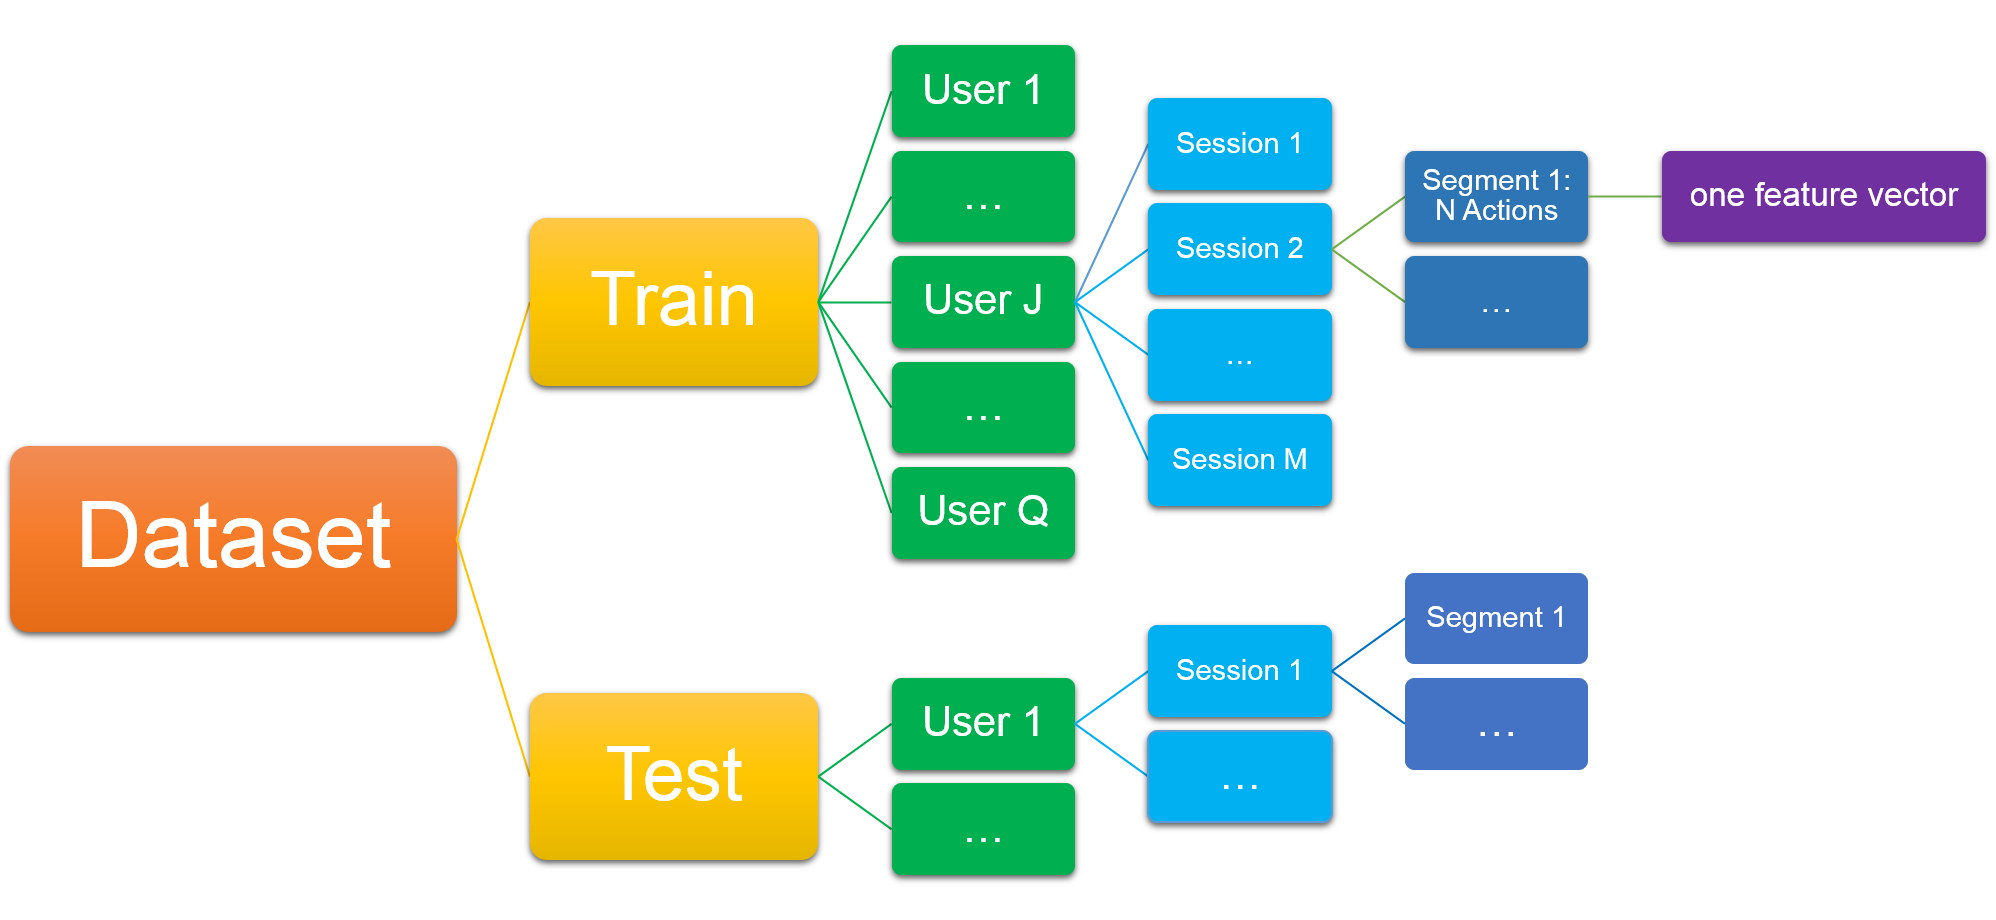
\includegraphics[width=\linewidth]{DataStructure.png}
        \caption{Структура данных}
        \label{sec:Research:Data:Description:fig:DataStructure}
    \end{figure}


    \subsubsection{Выявленные особенности данных}
    \label{sec:Research:Data:Features}
    
    Во время анализа данных были обнаружены следующие особенности:
    \begin{enumerate}
        \item Полностью дублирующиеся записи в таблице;
        \item Дубликаты временных меток;
        \item Множественные дубликаты положения мыши (зацикливание);
        \item Сверхбольшие значения координат;
        \item В датасете BALABIT:
        \begin{enumerate}
            \item В состоянии прокрутки колеса (Scroll) положение мыши перемещается в начало координат;
            \item Основная работа пользователей происходит в левом нижнем углу экрана.
        \end{enumerate}
    \end{enumerate}

    
    \subsection{Построение признакового пространства}
    
    \subsection{Построение модели пользователя}
    \subsubsection{OneClassSVM}
    \subsubsection{IsolationForest}
    \subsubsection{EllipticEnvelope}
    \subsubsection{LocalOutlierFactor}

    \newpage



    \section{Описание практической части}
    \label{sec:PracticalPart}

    \newpage



    \section{Планы на будущее}
    \label{sec:Future}

    \newpage



    \section{Заключение}
    \label{sec:Conclusion}

    \newpage



    \section{Список цитируемой литературы}
    \label{sec:ListOfReferences}
    \begin{enumerate}
        \item ...
        \item Fülöp, Á., Kovács, L., Kurics, T., Windhager-Pokol, E. (2016). Balabit Mouse Dynamics Challenge data set. Available at: https://github.com/balabit/Mouse-Dynamics-Challenge
        \item Harilal A. et al. Twos: A dataset of malicious insider threat behavior based on a gamified competition //Proceedings of the 2017 International Workshop on Managing Insider Security Threats. – 2017. – С. 45-56.
        \item ...
        \item Mondal S., Bours P. A study on continuous authentication using a combination of keystroke and mouse biometrics //Neurocomputing. – 2017. – Т. 230. – С. 1-22.
        \item Feher C. et al. User identity verification via mouse dynamics //Information Sciences. – 2012. – Т. 201. – С. 19-36.
    \end{enumerate}

    \newpage


\end{document}
